\documentclass[10pt,landscape,twocolumn,letterpaper]{article}

\usepackage[margin=1.27cm]{geometry}
\setlength{\textwidth}{10.0in}		% default=9in

\setlength{\columnsep}{0.5in}		% default=10pt
\setlength{\columnseprule}{0pt}		% default=0pt (no line)
%\setlength{\columnseprule}{0.2pt}		% default=0pt (no line)

\setlength{\textheight}{7in}		% default=5.15in
\setlength{\topmargin}{-.5in}		% default=0.20in

\setlength{\headsep}{0in}		% default=0.35in

\setlength{\parskip}{1.2ex}
\setlength{\parindent}{0mm}
\usepackage{graphicx}

%\usepackage{helvetica,color}
%\usepackage{newcent,color}
%\usepackage{bookman,color}
\usepackage{palatino}
\usepackage{color}
\usepackage{stmaryrd}
\pagestyle{empty}

\begin{document}
%\maketitle


\begin{center}
\textbf{Genesis}
\end{center}
Genesis is the book of beginnings.  It records not only the beginning of the heavens and the earth, and of plant, animal, and human life, but also of human institutions and relationships.  Typically, it speaks of the new birth, the new creation, where all was chaos and ruin.  With Genesis begins also the progressive self-revelation of God which culminates in Christ.  Three primary names of deity, Elohim Jehovah, and Adonai, and the five most important of the compound names, occur in Genesis; and that in an ordered progression which could not be changed without confusion.  The problem of sin as affecting man's condition in the earth, and his relation to God, and the divine solution of that problem are here in essence.  Of the eight great covenants which condition human life and the divine redemption, four, the Edenic, Adamic, Noahic, and Abrahamic Covenants, are in this book; and these four are the fundamental covenants to which the other four, the Mosaic, Palestinian, Davidic, and New Covenants, are related chiefly as adding detail or development.  Genesis enters into the very structure of the New Testament, in which it is quoted above sixty times in seventeen books.  In a profound sense, therefore, the roots of all subsequent revelation are planted deep in Genesis, and whoever would truly comprehend that revelation must begin here.

\begin{tabular}{p{0.7in}p{0.7in}p{1.8in}p{0.55in}}
  %\hline
  % after \\: \hline or \cline{col1-col2} \cline{col3-col4} ...
  DAY & CH & COMMENTS &  \\
\tiny 001 \normalsize \textcolor[rgb]{0.00,0.00,1.00}{Sat, $1^{st}$} & \textcolor[rgb]{0.00,0.00,1.00}{Gen 1-3} & \textcolor[rgb]{0.50,0.50,0.50}{\footnotesize Creation \& Fall} & $\boxempty$ $\boxempty$ $\boxempty$\\
\tiny 002 \normalsize \textcolor[rgb]{0.00,0.00,1.00}{Sun, $2^{nd}$} & \textcolor[rgb]{0.00,0.00,1.00}{Gen 4-6} & \textcolor[rgb]{0.50,0.50,0.50}{\footnotesize Civilization Through the Flood} & $\boxempty$ $\boxempty$ $\boxempty$\\
     & \multicolumn{2}{l}{\textcolor[rgb]{1.00,0.00,0.00}{Psalm 1 -- The Blessed Man}} & $\boxempty$ \\
\tiny 003 \normalsize \textcolor[rgb]{0.00,0.00,1.00}{Mon, $3^{rd}$} & \textcolor[rgb]{0.00,0.00,1.00}{Gen 7-9} & \textcolor[rgb]{0.50,0.50,0.50}{\footnotesize After the Flood} & $\boxempty$ $\boxempty$ $\boxempty$\\
\tiny 004 \normalsize \textcolor[rgb]{0.00,0.00,1.00}{Tue, $4^{th}$} & \textcolor[rgb]{0.00,0.00,1.00}{Gen 10-12} & \textcolor[rgb]{0.50,0.50,0.50}{\footnotesize Abraham} & $\boxempty$ $\boxempty$ $\boxempty$\\
     & \multicolumn{2}{l}{\textcolor[rgb]{1.00,0.00,0.00}{Psalm 2 -- The Heathen Rage \& the Lord Reigns}} & $\boxempty$ \\
\tiny 005 \normalsize \textcolor[rgb]{0.00,0.00,1.00}{Wed, $5^{th}$} & \textcolor[rgb]{0.00,0.00,1.00}{Gen 13-15} & \textcolor[rgb]{0.50,0.50,0.50}{\footnotesize Abraham, Lot \& the Covenant} & $\boxempty$ $\boxempty$ $\boxempty$\\
\tiny 006 \normalsize \textcolor[rgb]{0.00,0.00,1.00}{Thu, $6^{th}$} & \textcolor[rgb]{0.00,0.00,1.00}{Gen 16-18} & \textcolor[rgb]{0.50,0.50,0.50}{\footnotesize Ishmael}  & $\boxempty$ $\boxempty$ $\boxempty$\\
\tiny 007 \normalsize \textcolor[rgb]{0.00,0.00,1.00}{Fri, $7^{th}$} & \textcolor[rgb]{0.00,0.00,1.00}{Gen 19-21} & \textcolor[rgb]{0.50,0.50,0.50}{\footnotesize Sodom\& Gemorrah} & $\boxempty$ $\boxempty$ $\boxempty$\\
     & \multicolumn{2}{l}{\textcolor[rgb]{1.00,0.00,0.00}{Psalm 3 -- A Psalm of God's Protection}} & $\boxempty$ \\
\tiny 008 \normalsize \textcolor [rgb]{0.00,0.00,1.00}{Sat, $8^{th}$} & \textcolor[rgb]{0.00,0.00,1.00}{Gen 22-24} & \textcolor[rgb]{0.50,0.50,0.50}{\footnotesize Isaac \& His Marriage}  & $\boxempty$ $\boxempty$ $\boxempty$\\
\tiny 009 \normalsize \textcolor[rgb]{0.00,0.00,1.00}{Sun, $9^{th}$} & \textcolor[rgb]{0.00,0.00,1.00}{Gen 25-27} & \textcolor[rgb]{0.50,0.50,0.50}{\footnotesize Jacob and Esau}  & $\boxempty$ $\boxempty$ $\boxempty$\\
     & \multicolumn{2}{l}{\textcolor[rgb]{1.00,0.00,0.00}{Psalm 4 -- God Hears David's Call}} & $\boxempty$ \\
\tiny 010 \normalsize \textcolor[rgb]{0.00,0.00,1.00}{Mn, $10^{th}$} & \textcolor[rgb]{0.00,0.00,1.00}{Gen 28-30} & \textcolor[rgb]{0.50,0.50,0.50}{\footnotesize Jacob's Adventures}  & $\boxempty$ $\boxempty$ $\boxempty$\\
\tiny 011 \normalsize \textcolor[rgb]{0.00,0.00,1.00}{Tue, $11^{th}$} & \textcolor[rgb]{0.00,0.00,1.00}{Gen 31-33} & \textcolor[rgb]{0.50,0.50,0.50}{\footnotesize Jacob's Dream \&  Laban} & $\boxempty$ $\boxempty$ $\boxempty$\\
     & \multicolumn{2}{l}{\textcolor[rgb]{1.00,0.00,0.00}{Psalm 5 -- God's Hatred of Sin}} & $\boxempty$ \\
\tiny 012 \normalsize \textcolor[rgb]{0.00,0.00,1.00}{Wd, $12^{th}$} & \textcolor[rgb]{0.00,0.00,1.00}{Gen 34-36} & \textcolor[rgb]{0.50,0.50,0.50}{\footnotesize Jacob's Later Life} & $\boxempty$ $\boxempty$ $\boxempty$\\
\tiny 013 \normalsize \textcolor[rgb]{0.00,0.00,1.00}{Thu, $13^{th}$} & \textcolor[rgb]{0.00,0.00,1.00}{Gen 37-39} & \textcolor[rgb]{0.50,0.50,0.50}{\footnotesize The Story of Joseph}  & $\boxempty$ $\boxempty$ $\boxempty$\\
\tiny 014 \normalsize \textcolor[rgb]{0.00,0.00,1.00}{Fri, $14^{th}$} & \textcolor[rgb]{0.00,0.00,1.00}{Gen 40-42} & \textcolor[rgb]{0.50,0.50,0.50}{\footnotesize Joseph the Dream-man} & $\boxempty$ $\boxempty$ $\boxempty$\\
     & \multicolumn{2}{l}{\textcolor[rgb]{1.00,0.00,0.00}{Psalm 6 -- God's Use of David's Enemies}} & $\boxempty$ \\
\tiny 015 \normalsize   \textcolor[rgb]{0.00,0.00,1.00}{Sat, $15^{th}$} & \textcolor[rgb]{0.00,0.00,1.00}{Gen 43-45} & \textcolor[rgb]{0.50,0.50,0.50}{\footnotesize Joseph \& 11 Brothers} & $\boxempty$ $\boxempty$ $\boxempty$\\
\end{tabular}

\begin{tabular}{p{0.7in}p{0.7in}p{1.8in}p{0.55in}}
\tiny 016 \normalsize \textcolor[rgb]{0.00,0.00,1.00}{Sun, $16^{th}$} & \textcolor[rgb]{0.00,0.00,1.00}{Gen 46-48} &  & $\boxempty$ $\boxempty$ $\boxempty$\\
     & \multicolumn{2}{l}{\textcolor[rgb]{1.00,0.00,0.00}{Psalm 7 -- The First Imprecatory Psalm}} & $\boxempty$ \\
\tiny 017 \normalsize \textcolor[rgb]{0.00,0.00,1.00}{Mn, $17^{th}$} & \textcolor[rgb]{0.00,0.00,1.00}{Gen 49-50} &  & $\boxempty$ $\boxempty$\\
\end{tabular}

\begin{center}
\textbf{Exodus}
\end{center}
Exodus, ``going out,'' records the redemption out of Egyptian bondage of the descendants of Abraham, and sets forth, in type, all redemption. It is therefore peculiarly the book of redemption.  But as all redemption is unto a relationship with God of which worship, fellowship, and service are expressions, so Exodus, in the giving of the law and the provisions of sacrifice and priesthood, becomes not only the book of redemption, but also, in type, of the conditions upon which all relationships with God exist.  Broadly, the book teaches that redemption is essential to any relationship with a holy God; and that even a redeemed people cannot have fellowship with Him unless constantly cleansed from defilement.  In Exodus, God, hitherto connected the Israelitish people only through His covenant with Abraham, brings them to Himself \emph{nationally} through redemption, puts them under the Mosaic covenant, and dwells among them in the cloud of glory.  Galatians explains the relation of the law to the Abrahamic covenant.  In the Commandments God taught Israel His just demands.

\begin{tabular}{p{0.7in}p{0.7in}p{1.8in}p{0.55in}}
  %\hline
  % after \\: \hline or \cline{col1-col2} \cline{col3-col4} ...
  DAY & CH & COMMENTS &  \\
\tiny 018 \normalsize \textcolor[rgb]{0.00,0.00,1.00}{Tue, $18^{th}$} & \textcolor[rgb]{0.00,0.00,1.00}{Exo 1-3} & \textcolor[rgb]{0.50,0.50,0.50}{\footnotesize Moses' Early Days} & $\boxempty$ $\boxempty$ $\boxempty$\\
     &  \multicolumn{2}{l}{\textcolor[rgb]{1.00,0.00,0.00}{Psalm 8 -- A Hymn of Praise}} & $\boxempty$ \\
\tiny 019 \normalsize \textcolor[rgb]{0.00,0.00,1.00}{Wd, $19^{th}$} & \textcolor[rgb]{0.00,0.00,1.00}{Exo 4-6} & \textcolor[rgb]{0.50,0.50,0.50}{\footnotesize Moses Goes to Pharaoh} & $\boxempty$ $\boxempty$ $\boxempty$\\
\tiny 020 \normalsize \textcolor[rgb]{0.00,0.00,1.00}{Thu, $20^{th}$} & \textcolor[rgb]{0.00,0.00,1.00}{Exo 7-9} & \textcolor[rgb]{0.50,0.50,0.50}{\footnotesize Plagues 1-7} & $\boxempty$ $\boxempty$ $\boxempty$\\
\tiny 021 \normalsize \textcolor[rgb]{0.00,0.00,1.00}{Fri, $21^{st}$} & \textcolor[rgb]{0.00,0.00,1.00}{Exo 10-12} & \textcolor[rgb]{0.50,0.50,0.50}{\footnotesize Passover \& Departure} & $\boxempty$ $\boxempty$ $\boxempty$\\
     & \multicolumn{2}{l}{\textcolor[rgb]{1.00,0.00,0.00}{Psalm 9 -- Praising the Righteous Judge}} & $\boxempty$ \\
\tiny 022 \normalsize   \textcolor[rgb]{0.00,0.00,1.00}{Sat, $22^{nd}$} & \textcolor[rgb]{0.00,0.00,1.00}{Exo 13-15} & \textcolor[rgb]{0.50,0.50,0.50}{\footnotesize Deliverance \& First Dissatisfaction} & $\boxempty$ $\boxempty$ $\boxempty$\\
\tiny 023 \normalsize \textcolor[rgb]{0.00,0.00,1.00}{Sun, $23^{rd}$} & \textcolor[rgb]{0.00,0.00,1.00}{Exo 16-18} & \textcolor[rgb]{0.50,0.50,0.50}{\footnotesize Division of Responsibility} & $\boxempty$ $\boxempty$ $\boxempty$\\
     & \multicolumn{2}{l}{\textcolor[rgb]{1.00,0.00,0.00}{Psalm 10 -- A Psalm of Deliverance}} & $\boxempty$ \\
\tiny 024 \normalsize \textcolor[rgb]{0.00,0.00,1.00}{Mn, $24^{th}$} & \textcolor[rgb]{0.00,0.00,1.00}{Exo 19-21} & \textcolor[rgb]{0.50,0.50,0.50}{\footnotesize Giving of the Law} & $\boxempty$ $\boxempty$ $\boxempty$\\
\tiny 025 \normalsize \textcolor[rgb]{0.00,0.00,1.00}{Tue, $25^{th}$} & \textcolor[rgb]{0.00,0.00,1.00}{Exo 22-24} & \textcolor[rgb]{0.50,0.50,0.50}{\footnotesize Giving of the Law} & $\boxempty$ $\boxempty$ $\boxempty$\\
     & \multicolumn{2}{l}{\textcolor[rgb]{1.00,0.00,0.00}{Psalm 11 -- A Psalm of Trust}} & $\boxempty$ \\
\tiny 026 \normalsize \textcolor[rgb]{0.00,0.00,1.00}{Wd, $26^{th}$} & \textcolor[rgb]{0.00,0.00,1.00}{Exo 25-27} & \textcolor[rgb]{0.50,0.50,0.50}{\footnotesize Institution of the Tabernacle} & $\boxempty$ $\boxempty$ $\boxempty$\\
\tiny 027 \normalsize \textcolor[rgb]{0.00,0.00,1.00}{Thu, $27^{th}$} & \textcolor[rgb]{0.00,0.00,1.00}{Exo 28-30} & \textcolor[rgb]{0.50,0.50,0.50}{\footnotesize Priests \& the Altar} & $\boxempty$ $\boxempty$ $\boxempty$\\
\tiny 028 \normalsize \textcolor[rgb]{0.00,0.00,1.00}{Fri, $28^{th}$} & \textcolor[rgb]{0.00,0.00,1.00}{Exo 31-33} & \textcolor[rgb]{0.50,0.50,0.50}{\footnotesize Moses \& the Commandments} & $\boxempty$ $\boxempty$ $\boxempty$\\
     & \multicolumn{2}{l}{\textcolor[rgb]{1.00,0.00,0.00}{Psalm 12 -- Preservation of God's Words}} & $\boxempty$ \\
\tiny 029 \normalsize    \textcolor[rgb]{0.00,0.00,1.00}{Sat, $29^{th}$} & \textcolor[rgb]{0.00,0.00,1.00}{Exo 34-36} & \textcolor[rgb]{0.50,0.50,0.50}{\footnotesize Covenant \& Construction Begins} & $\boxempty$ $\boxempty$ $\boxempty$\\
\tiny 030 \normalsize \textcolor[rgb]{0.00,0.00,1.00}{Sun, $30^{th}$} & \textcolor[rgb]{0.00,0.00,1.00}{Exo 37-40} & \textcolor[rgb]{0.50,0.50,0.50}{\footnotesize Construction of Tabernacle} & $\boxempty$ $\boxempty$ $\boxempty$ $\boxempty$\\
     & \multicolumn{2}{l}{\textcolor[rgb]{1.00,0.00,0.00}{Psalm 13 -- God Delivers from Oppression}} & $\boxempty$ \\
\end{tabular}






\begin{center}
\textbf{Leviticus}
\end{center}
Leviticus stands in the same relation to Exodus, that the Epistles do to the Gospels.  Exodus is the record of redemption, and lays the foundation of the cleansing, worship, and service of a redeemed people.  Leviticus gives the detail of the walk, worship, and service of that people.  In Exodus God speaks out of the mount to which approach was forbidden; in Leviticus He speaks out of the tabernacles in which He dwells in the midst of His people, to tell them that which befits His holiness in their approach to, and communion with, Himself.  The key-word of Leviticus is holiness, occurring 87 times. Key-verse, 19:2.  Leviticus is in nine chief divisions: I. The Offering, 1:1 - 6:7.  II. The Law of the Offerings 6:8 - 7:38. III. Consecration, 8:1 - 9:24. IV. A Warning Example, 10:1 - 20.  V. A Holy God must have a Cleansed People, 11:1 - 15. VI. Atonement, 16 - 17. VII.  The Relationships of God's People, 18 - 22.  VIII. The Feasts of Jehovah, 23. IX. Instructions and Warnings, 24 - 27.

\begin{tabular}{p{0.7in}p{0.7in}p{1.8in}p{0.55in}}
  %\hline
  % after \\: \hline or \cline{col1-col2} \cline{col3-col4} ...
  DAY & CH & COMMENTS &  \\
\tiny 031 \normalsize \textcolor[rgb]{0.00,0.00,1.00}{Mon, $31^{st}$} & \textcolor[rgb]{0.00,0.00,1.00}{Lev 1-3} &  \textcolor[rgb]{0.50,0.50,0.50}{\footnotesize Burnt, Meal \& Peace Offerings} & $\boxempty$ $\boxempty$ $\boxempty$\\
\end{tabular}






\newpage
\LARGE
\begin{center}
\textcolor[rgb]{0.98,0.00,0.00}{Daily Bible Reading}\\
\textcolor[rgb]{0.00,0.00,1.00}{January 2022}\\
\end{center}


\begin{figure}[htp]
    \centering
  % Requires \usepackage{graphicx}
%  \includegraphics[width=4.5in]{LBT-December-Bible-Reading-Schedule.jpg}\\
  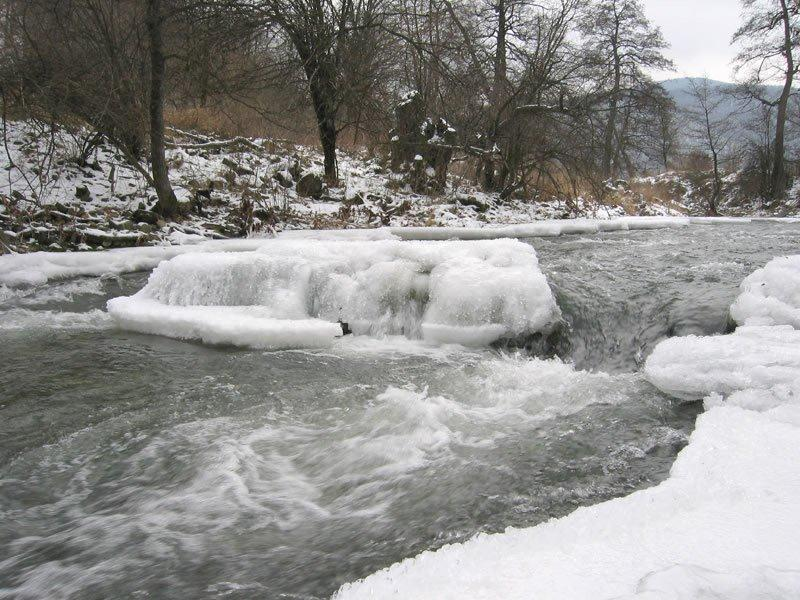
\includegraphics[width=4.5in]{January.jpg}\\
%  \caption{}\label{}
\end{figure}

\begin{center}
\textcolor[rgb]{0.00,0.00,1.00}{\\Ask Yourself ...}
\textcolor[rgb]{1.00,0.00,0.00}{\\Who is Speaking?\\Who is being spoken to?\\What is being said?\\Are there
any commandments to obey?\\Are there any promises to claim?}
\end{center}

\end{document}
